% =================================================================================================
% File:			appendici.tex
% Description:	Definisce le appendici riguardanti gli standard di qualità
% Created:		2014/01/11
% Author:		Ceccon Lorenzo
% Email:		ceccon.lorenzo@mashup-unipd.it
% =================================================================================================
% Modification History:
% Version		Modifier Date		Change											Author
% 0.0.1 		2014/01/11 			iniziata stesura appendice					Lorenzo C.
% =================================================================================================
%

% CONTENUTO DEL CAPITOLO

\appendix 

\section{Modelli e standard di qualità}
  	\subsection{Standard ISO/IEC 9126}
  	Lo standard ISO/IEC 9126 è uno standard creato per delineare delle normative utili a descrivere un modello di qualità del software. Lo standard propone un approccio in cui viene posta attenzione al miglioramento dell'organizzazione e dei processi di una società di software, in modo da migliorare di conseguenza la qualità del prodotto software.\\
  	\begin{figure}[h]
		\centering
		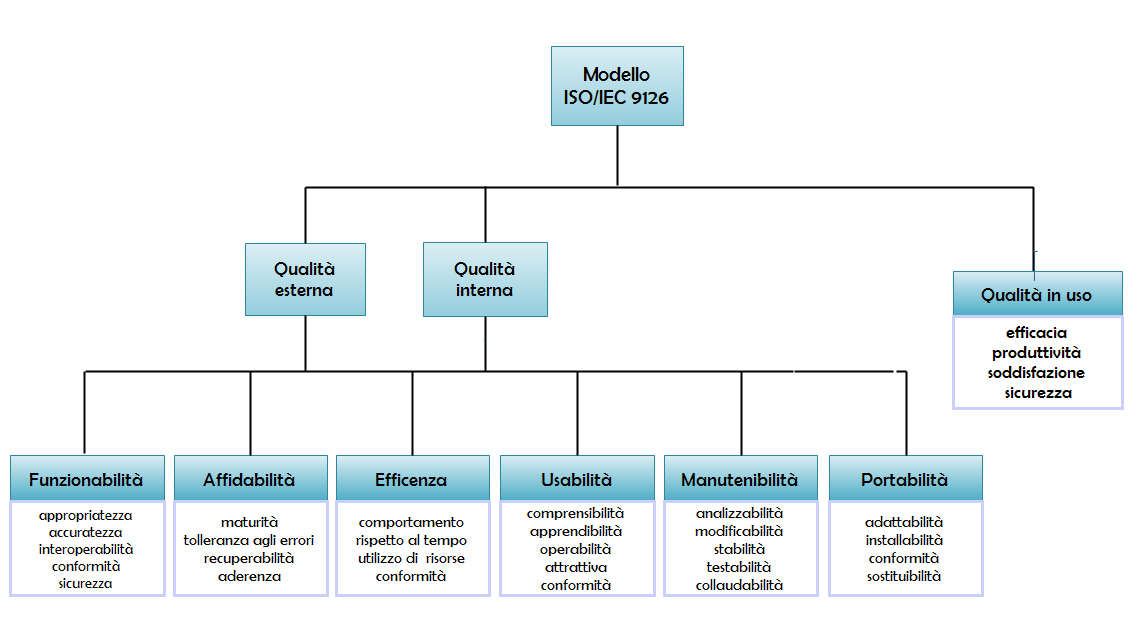
\includegraphics[width=140mm]{images/iso_9126.png}
		\caption{Schema del modello di qualità ISO/IEC 9126}
		\label{fig:iso9126}
	\end{figure}
  	Lo standard ISO/IEC 9126 è suddiviso in quattro parti:
		\begin{itemize}
			\item \textbf{Modello di qualità: } la prima parte dello standard classifica il modello di qualità in sei caratteristiche generali e in varie sotto caratteristiche misurabili tramite l'utilizzo di metriche.\\
			Le sei caratteristiche generali e le relative sotto caratteristiche sono:
				\begin{itemize}
					\item \textbf{Funzionalità:} capacità di un prodotto software di fornire funzioni che soddisfano esigenze stabilite
						\begin{itemize}
							\item \textbf{Appropriatezza:} capacità del prodotto software di fornire un appropriato insieme di funzioni per i specifici compiti ed obiettivi prefissati all'utente;
							\item \textbf{Accuratezza:} capacità del prodotto software di fornire i risultati richiesti;
							\item \textbf{Interoperabilità:} capacità del prodotto software di interagire con i diversi sistemi specificati;
							\item \textbf{Conformità:} capacità del prodotto software di aderire agli standard e alle convenzioni appartenenti al settore in cui vengono applicati;
							\item \textbf{Sicurezza:} capacità del prodotto software di consentire l'accesso a dati e informazioni solamente alle persone autorizzate.
						\end{itemize}
					\item \textbf{Affidabilità:} capacità del prodotto software di mantenere uno specificato livello di prestazioni
						\begin{itemize}
							\item \textbf{Maturità:} capacità di un software di evitare che si verificano errori, malfunzionamenti o siano prodotti risultati non corretti;
							\item \textbf{Tolleranza agli errori:} capacità del software di mantenere un adeguato livello di prestazioni in presenza di malfunzionamenti;
							\item \textbf{Recuperabilità:} capacità di un prodotto di ripristinare il livello appropriato di prestazioni in seguito a un malfunzionamento;
							\item \textbf{Aderenza:} capacità di aderire a standard, regole e convenzioni inerenti all'affidabilità.
						\end{itemize}
					\item \textbf{Usabilità:} capacità del software di essere capito, appreso e usato dall'utente
						\begin{itemize}
							\item \textbf{Comprensibilità:} esprime la facilità di comprensione delle funzionalità del prodotto;
							\item \textbf{Apprendibilità:} capacità del software di essere appreso in tempo brevi;
							\item \textbf{Operabilità:} capacità di permettere agli utenti di utilizzare al software al fine di raggiungere i propri scopi;
							\item \textbf{Attrattiva:} capacità del prodotto di risultare interessante all'utente;
							\item \textbf{Conformità:} capacità del software di aderire a standard, regole e convenzioni relativi all'usabilità.
						\end{itemize}
					\item \textbf{Efficienza:} capacità di fornire prestazioni relativamente alla quantità di risorse usate
						\begin{itemize}
							\item \textbf{Comportamento rispetto al tempo:} capacità di fornire tempi di risposta, elaborazione e velocità di attraversamento ottimali in relazione alla funzione utilizzata;
							\item \textbf{Utilizzo delle risorse:} capacità del software di utilizzare adeguate quantità di risorse;
							\item \textbf{Conformità:} capacità del software di aderire a standard, regole e convenzioni relativi all'efficienza.
						\end{itemize}
					\item \textbf{Manutenibilità:} capacità del software di essere modificato apportando correzioni, miglioramenti o adattamenti
						\begin{itemize}
							\item \textbf{Analizzabilità:} esprime la facilità nell'analizzare il codice sorgente per ricercare errori; 
							\item \textbf{Modificabilità:} capacità del software di permettere l'implementazione di nuove modifiche;
							\item \textbf{Stabilità:} capacità del software di evitare effetti indesiderati a seguito di modifiche errate;
							\item \textbf{Testabilità:} capacità del software di eseguire facilmente la validazione delle modifiche apportate al software.
						\end{itemize}
					\item \textbf{Portabilità:} capacità del software di lavorare in diversi ambienti di lavoro
						\begin{itemize}
							\item \textbf{Adattabilità:} capacità del software di essere adattato a diversi ambienti senza dover applicare modifiche diverse da quelle fornite;
							\item \textbf{Installabilità:} capacità del software di essere installato in uno specificato ambiente;
							\item \textbf{Conformità:} capacità del prodotto software di aderire a standard, regole e convenzioni relativi alla portabilità;
							\item \textbf{Sostituibilità:} capacità del software di sostituire un altro software analogo per svolgere certi compiti.
						\end{itemize}
				\end{itemize}
			\item \textbf{Qualità esterne: } le metriche esterne applicabili al software, e quindi rilevabili tramite l'analisi dinamica, misurano i comportamento del prodotto sulla base dei test, dall'operatività e dall'osservazione durante la sua esecuzione;
			\item \textbf{Qualità interne: } le metriche interne, misurabili attraverso l'analisi statica, sono utili per prevedere il livello della qualità esterna ed in uso, poiché i suoi attributi interni influiscono su quelli esterni ed in uso. Permettono così di individuare anomalie prima che queste ultime possano influenzare la qualità del prodotto finale;
			\item \textbf{Qualità in uso: } la qualità in uso, raggiungibile solo dopo aver ottenuto la qualità interna ed esterna, fornisce metriche per misurare il grado di utilizzabilità del prodotto da parte dell'utente finale.
		\end{itemize}
		
	\subsection{Standard ISO/IEC 15504}
	Lo standard ISO/IEC 15504, conosciuto anche come SPICE, è un insieme di documenti tecnici per lo sviluppo di processi software, utili a valutare la dimensione dei processi tramite l'utilizzo di specifiche metriche. É derivato dallo standard ISO/IEC 12207 e da modelli di maturità quali Bootstrap, Trillium e il CMM.\\
	Lo standard definisce la dimensione del processo e la suddivide nelle seguenti cinque categorie:
		\begin{itemize}
			\item \textbf{Custormer/Supplier;}
			\item \textbf{Engineering;}
			\item \textbf{Support;}
			\item \textbf{Management;}
			\item \textbf{Organization.}
		\end{itemize}
	Per ogni processo, viene definito un livello di capacità dei processi definito da una scala di sei livelli e da nove attributi suddivisi nei vari livelli:
		\begin{itemize}
			\item \textbf{Level 5. Optimizing process:} il processo è predicibile ed in grado di adattarsi per raggiungere
obiettivi specifici
				\begin{itemize}
					\item \textbf{Process Innovation:} le modifiche ad un processo sono identificate ed implementate al fine di ottenere il miglioramento continuo nel raggiungimento degli obiettivi;
					\item \textbf{Process Optimization:} le modifiche alla definizione, gestione, attuazione di un processo sono controllate.
				\end{itemize}
			\item \textbf{Level 4. Predictable process:} il processo è stabilizzato ed è attuato all'interno di definiti limiti di controllo
				\begin{itemize}
					\item \textbf{Process Measurement:} i risultati raggiunti e le misure rilevate durante l'attuazione di un processo sono utilizzati per garantire il raggiungimento di specifici obiettivi;
					\item \textbf{Process Control:} un processo è controllato attraverso le misure di prodotto e di processo rilevate, al fine di migliorare le modalità di attuazione del processo stesso.
				\end{itemize}
			\item \textbf{Level 3. Established process:} il processo è attuato, pianificato e controllato sulla base di procedure standard basate sui principi dell'ingegneria del software
				\begin{itemize}
					\item \textbf{Process Definition:} l'attuazione di un processo, per raggiungere gli obiettivi, si basa sull'adozione di approcci standard;
					\item \textbf{Process Deployment:} l'attuazione di un processo, per raggiungere gli obiettivi, fa uso di risorse umane e tecniche appropriate.
				\end{itemize}
			\item \textbf{Level 2. Managed process:} il processo è attuato ma anche pianificato, tracciato, verificato ed aggiustato se necessario, sulla base di obiettivi ben definiti
				\begin{itemize}
					\item \textbf{Performance Management:} l'implementazione di un processo è pianificato e controllato al fine di produrre risultati coerenti agli obiettivi attesi;
					\item \textbf{Work Product Management:} l'implementazione di un processo è pianificato e controllato al fine di produrre risultati documentati, controllati e verificati in modo appropriato.
				\end{itemize}			
			\item \textbf{Level 1. Performed process:} il processo viene messo in atto e raggiunge i suoi obiettivi. Il risultato potrebbe non essere stato pianificato e tracciato rigorosamente
				\begin{itemize}
					\item \textbf{Process Performance:} capacità di un processo di raggiungere i suoi obiettivi trasformando input identificabili in output identificabili.
				\end{itemize}
			\item \textbf{Level 0. Incomplete process:} il processo non è stato implementato oppure non raggiunge gli obiettivi.
		\end{itemize}
	Ogni attributo è misurabile tramite l'utilizzo di una scala di valutazione divisa in quattro punti:
		\begin{itemize}
			\item \textbf{Not achieved (0-15\%);}
			\item \textbf{Partially achieved (15-50\%);}
			\item \textbf{Largely achieved (50-85\%);}
			\item \textbf{Fully achieved (85-100\%).}
		\end{itemize}
	Lo standard fornisce una guida per l'effettuazione di una valutazione formata da:
		\begin{itemize}
			\item Processo di valutazione;
			\item Modello per la valutazione;
			\item Strumenti per la valutazione.
		\end{itemize}
	Lo standard infine, stabilisce che per una corretta valutazione i verificatori debbano avere un buon livello di competenza e di esperienza.
	
	\subsection{Ciclo PDCA}
	Il ciclo PDCA, noto anche come ciclo di Deming, è un metodo di gestione iterativo a quattro fasi per il controllo e il miglioramento continuo dei processi.\\
	Le quattro fasi che lo compongono sono:
			\begin{itemize}
				\item \textbf{Plan:} stabilisce gli obiettivi e i processi necessari per ottenere risultati uguali a quelli attesi;
				\item \textbf{Do:} fase composta dall'attuazione del piano, dall'esecuzione del processo e dalla creazione del prodotto. Termina con una raccolta dei dati e creazione di grafici sul risultato di quanto ottenuto;
				\item \textbf{Check:} si confrontano i risultati ottenuti dalla fase precedente con i risultati stabiliti durante la pianificazione per verificare la presenza di differenze;
				\item \textbf{Act:} si effettuano correzioni laddove sono presenti differenze tra i risultati ottenuti e quelli previsti. Si determinano le cause delle discrepanze e dove c'è bisogno di applicare delle modifiche per ottenere un miglioramento del processo e di conseguenza del prodotto.
			\end{itemize}
			\begin{figure}[h]
				\centering
				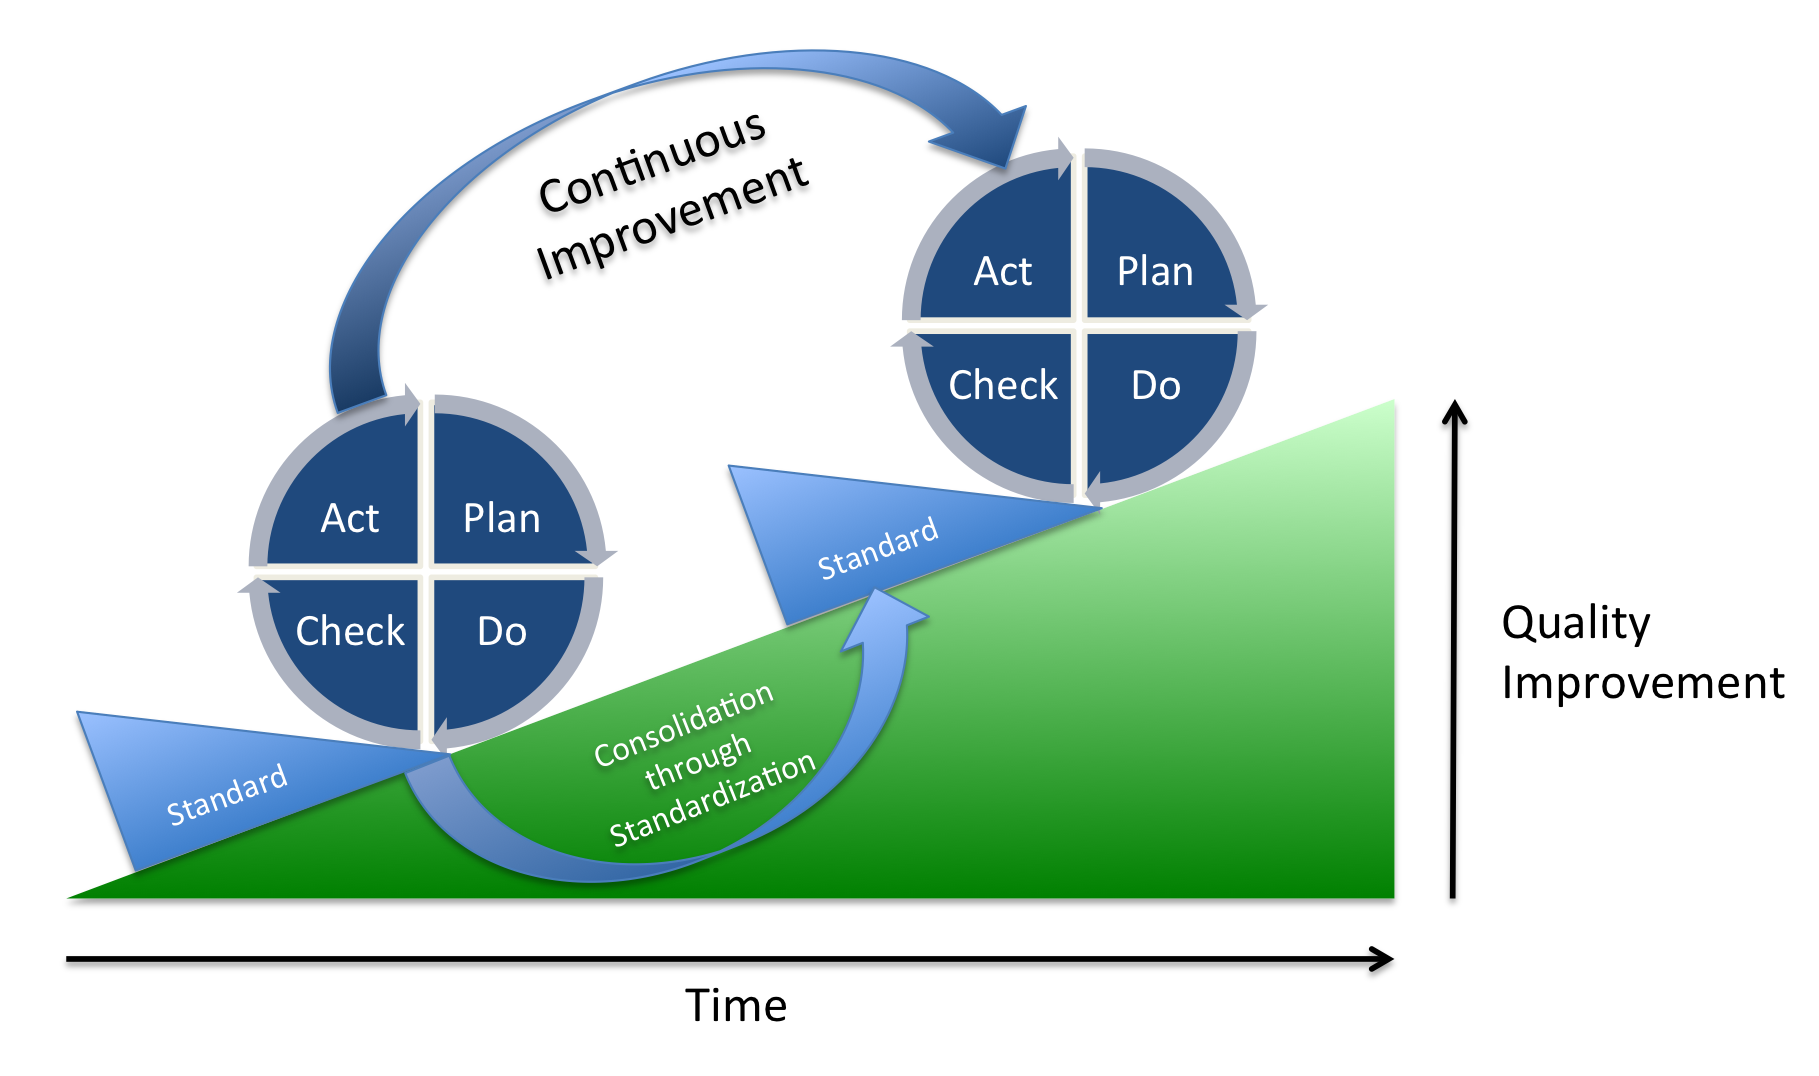
\includegraphics[width=120mm]{images/pdca.png}
				\caption{Ciclo di miglioramento della qualità PDCA}
				\label{fig:pdca}
			\end{figure}
		


\pagebreak
\section{Resoconto delle attività di verifica}
	\subsection{Revisione dei Requisiti}
	Nel periodo precedente alla consegna della \RR{} sono state effettuate delle attività di verifica sia per i documenti sia per i processi.\\
	Per quanto riguarda la verifica dei documenti si è effettuata attività di analisi statica descritta nelle \docNameVersionNdP. Inizialmente si è fatto uso della tecnica 	walkthrough per individuare gli errori. Dopodiché sono state avviate le procedure per la segnalazione e la gestione degli errori rilevati descritte nelle \docNameVersionNdP.
	In seguito si è proceduto a:
	\begin{itemize}
		\item correggere gli errori rilevati;
		\item compilare la lista di controllo utilizzando l'apposita sezione \emph{Bug Tracking Document} di Asana.
	\end{itemize}
	Una volta compilata la lista di controllo si è cominciato ad utilizzare la tecnica inspection.\\
	Si è quindi applicato il ciclo PDCA per migliorare i processi che hanno generato gli errori. Infine si sono applicate le metriche per i documenti descritte nella sezione 2.8.2 riportando i risultati nella sezione C dell'appendice di questo documento.
	Per quanto riguarda la verifica dei processi si sono svolte le attività descritte nelle \docNameVersionNdP{}. Si sono quindi applicate le metriche per i processi descritte nella sezione 2.8.1 di questo documento riportando i risultati nella sezione C dell'appendice di questo documento.
	\subsection{Revisione di Progettazione}
	TO DO
\pagebreak

\section{Dettaglio delle verifiche tramite analisi}
	\subsection{Ricerca ed implementazione degli strumenti}
		\subsubsection{Processi}
		Vengono qui riportati i valori degli indici di budget e schedule variance per le attività della fase \textbf{Ricerca ed implementazione degli strumenti}.
			\begin{table}[!ht]
			\begin{center}
				\begin{tabularx}{0.9\textwidth}{|l|l|X|}
					\hline
					\textbf{Attività} & \textbf{Schedule variance} & \textbf{Budget variance}\\
					\hline						
					\docNameVersionAdR & ?? & ??\\
					\hline
					\docNameVersionGlo & ?? & ??\\
					\hline					
					\docNameVersionNdP & ?? & ??\\
					\hline					
					\docNameVersionPdP & ?? & ??\\
					\hline					
					\docNameVersionPdQ & ?? & ??\\
					\hline					
					\docNameVersionSdF & ?? & ??\\
					\hline				
				\end{tabularx}
			\end{center}
		\caption{Esiti verifica sui processi fase - Ricerca ed implementazione degli strumenti}
	\end{table}
	Complessivamente si registrano:
	\begin{itemize}
	\item \textbf{Schedule variance:} ;
	\item \textbf{Budget variance:} .
	\end{itemize}
	Dai valori presentati si può dedurre che i periodi di slack introdotti aiutano ad avere una schedule variance positiva. L'inesperienza del gruppo invece ha fatto si che la budget variance sia negativa ma comunque non compromettente in quanto al di sopra del minimo accettabile di...



 	\subsubsection{Documenti}
		\begin{table}[!ht]
			\begin{center}
				\begin{tabularx}{0.9\textwidth}{|l|l|X|}
					\hline
					\textbf{Nome documento} & \textbf{Valore indice} & \textbf{Esito}\\
					\hline						
					\docNameVersionAdR & 56 & \textcolor{green}{Superato}\\
					\hline
					\docNameVersionGlo & 50 & \textcolor{green}{Superato}\\
					\hline					
					\docNameVersionNdP & 54 & \textcolor{green}{Superato}\\
					\hline					
					\docNameVersionPdP & 55 & \textcolor{green}{Superato}\\
					\hline					
					\docNameVersionPdQ & 55 & \textcolor{green}{Superato}\\
					\hline					
					\docNameVersionSdF & 48 & \textcolor{green}{Superato}\\
					\hline				
				\end{tabularx}
			\end{center}
			\caption{Risultati indice Gulpease}
		\end{table}
			
\pagebreak

\section{Esito delle revisioni}
In questa sezione verranno riportate un elenco delle modifiche per ogni documento apportate dal gruppo a seguito delle valutazioni fatte dal committente alle revisioni.\\
Viene qui sotto riportata una lista con tutte le modifiche effettuate divise per ogni revisione a cui il gruppo ha preso parte.

	\subsection{Revisione dei Requisiti}
	\begin{itemize}
		\item \textbf{\docNameAdR:} TO DO
		\item \textbf{\docNameNdP:} TO DO
		\item \textbf{\docNamePdP:} TO DO
		\item \textbf{\docNamePdQ:} TO DO
	\end{itemize}

\pagebreak